\documentclass[PICOAPC.tex]{subfiles}

\begin{document}

\subsection{Gravitational Waves and Inflation}
\label{sec:inflation}

Measurements of the \ac{CMB} $BB$ angular power spectrum are the only foreseeable way to detect  inflationary gravitational waves. The strength of the signal, quantified by the tensor-to-scalar ratio $r$, is a direct measure of the expansion rate of the Universe during inflation, and together with the Friedmann equation, it reveals the energy scale of inflation. A detection of $r$  ``would be a watershed discovery'', a quote from the 2010 decadal panel report~\citep{blandford2010}. 
%\comred{do you need to explain what BB is?}

PICO will detect primordial gravitational waves if inflation occurred at an energy scale of at least $5\times 10^{15}\,\rm{GeV}$, or equivalently $r= 5\times 10^{-4} \, (5\sigma)$.  In a community white paper setting targets for measurements of inflationary gravitational waves in the next decade, \citet{Shandera_etal} quote two theoretically motivated targets: (1) rejecting $r=0.01$, and (2) rejecting $r=0.001$. The second threshold is motivated by the goal of rejecting all inflationary models that naturally explain the observed value of the spectral index of primordial fluctuations $n_{\rm s}$ and having a characteristic scale in the potential that is larger than the Planck scale. 
They write "If these thresholds are passed without a detection, most textbook models of inflation will be ruled out; and, while the possibility of an early inflationary phase would still remain viable, the data would then force a significant change in our understanding of the primordial Universe." PICO is the only next decade experiment with the raw sensitivity to reject both targets at high confidence; see Figure~\ref{fig:nsr}. It is the only next decade experiment that can detect inflationary models that have $r \geq 5\times 10^{-4}$ at high confidence. 

%A detection will provide evidence for a new energy scale tantalizingly close to the energy scale associated with grand unified theories, probe physics at energies far beyond the reach of terrestrial colliders, and be the first observation of a phenomenon associated with quantum gravity~\cite{Krauss:2013pha}. 

%There are only two classes of slow-roll inflation in agreement with current data that naturally explain the observed value of the spectral index of primordial fluctuations $n_{\rm s}$~\cite{Aghanim:2018eyx}. The first class is characterized by potentials of the form $V(\phi)\propto\phi^p$. The second class is characterized by potentials that approach a constant as a function of field value, either like a power law or exponentially. All models in this class, with a characteristic scale in the potential that is larger than the Planck scale, predict a tensor-to-scalar ratio of $r\gtrsim 0.001$.

%With its strong constraints on $r$, the strongest anticipated among any proposed next decade experiment, PICO will either detect gravitational waves from either of these classes with high confidence, or it will be the only experiment to answer the challenge articulated by the recent `Inflationary Gravitational Waves' community science paper: "If these thresholds are passed without a detection, most textbook models of inflation will be ruled out; and, while the possibility of an early inflationary phase would still remain viable, the data would then force a significant change in our understanding of the primordial Universe."~\cite{Shandera_etal}.


%The simplest models of inflation, in which there is a single inflaton field, predict primordial fluctuations that are very nearly Gaussian with $|f^{\rm local}_{\rm NL}| <1$, where $f^{\rm local}_{\rm NL}$ is a parameter quantifying the level of local non-Gaussianity~\citep{planck2015_17}. A detection of $|f^{\rm local}_{\rm NL}| >1$ points exclusively to models of inflation with multiple fields (Fig.~\ref{fig:fnlconstraint}). 
%For $f^{\rm local}_{\rm NL}=2$, $3\sigma$ evidence will be reached through correlations between the PICO lensing potential maps (\S~\ref{sec:gravitationallensing}) and LSST galaxies. If LSST's auto-correlation can only be used on smaller angular scales $L\ge 20$, the $3\sigma$ evidence weakens to $2\sigma$. 

%\begin{figure}[!thb]
%\centering
%\vspace{-0.05in}
%\hspace{-0.15in}
%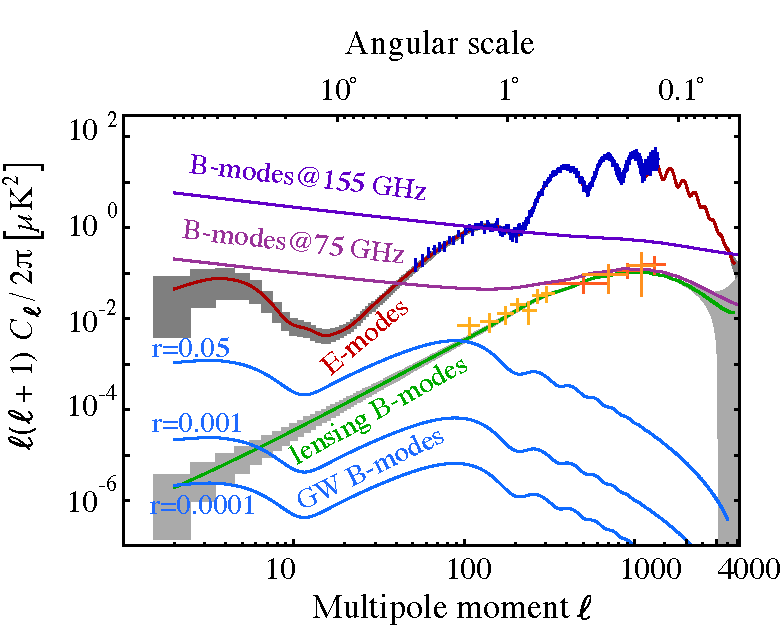
\includegraphics[width=3in]{images/cmb_powspec_PICOv4p1_v2.pdf}
%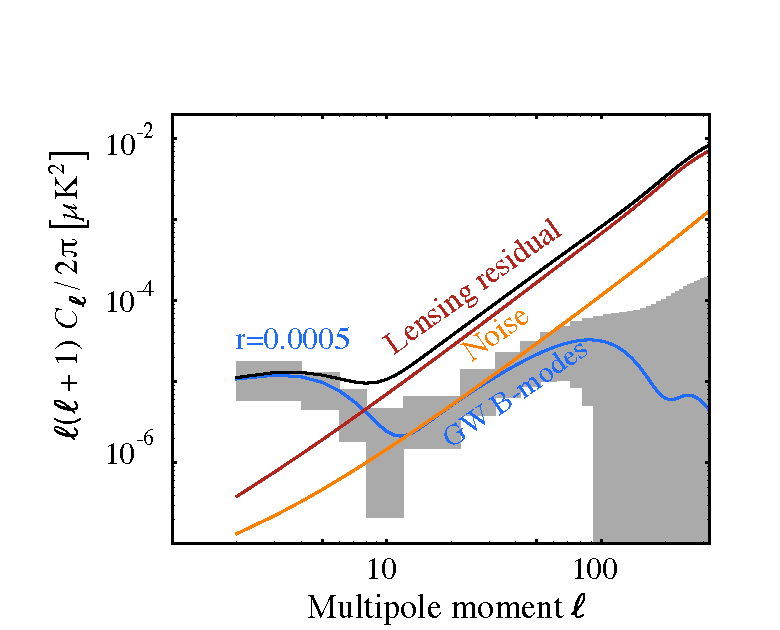
\includegraphics[width=3in]{images/cmbbb_powspec_PICOv4p1_v4.pdf}
%\vspace{-0.1in}
%\caption{\captiontext With PICO's baseline configuration we will measure the $EE$ (left, red) and lensing $BB$ (green) angular power spectra with high precision (grey). PICO's goal is to detect $r= 5\times 10^{-4}\, (5\sigma)$ (right, grey). This forecast includes PICO's 80\% delensing (red) and foreground separation. The baseline noise level (right, orange) allows detection of even lower levels; we expect foreground separation to limit performance.  As an example we show the total $BB$ spectra on the cleanest $60\%$ of the sky at 75 and 155~GHz (left, purple). The foregrounds largely dominate the cosmological signals. Also shown are measurements of lensing from current experiments (left, orange)~\citep{PB_BB, keisler2015, actpol_lensing_BB, Array:2015xqh}, \planck 's $EE$ measurements (left, dark blue)~\citep{Planck2018_I}, and the $BB$ spectrum produced by an inflationary gravity wave (GW) signal with different values of $r$ (cyan). 
%\label{fig:clbb} }
%\vspace{-0.05in}
%\end{figure}

\begin{figure}[!thb]
\parbox{4.5in}{\centerline{
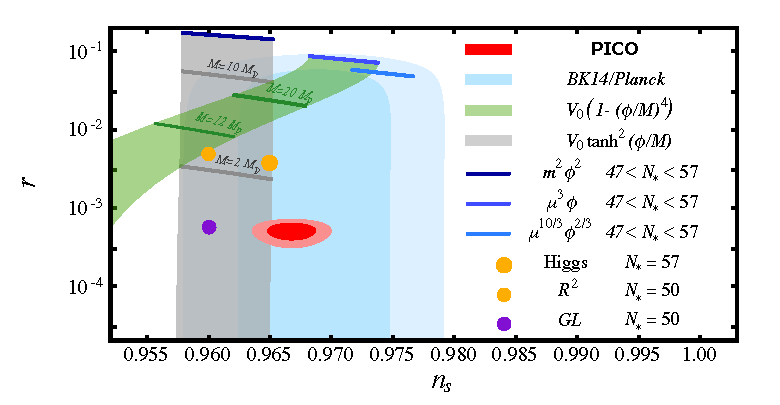
\includegraphics[width=4.5in]{images/nsrlabeledrp0005_PICOv2.pdf} } }
\parbox{1.8in}{
\caption{\captiontext  Current $1\sigma$ and 2$\sigma$ limits on $r$ and $n_{\rm s}$ (cyan) and forecasted constraints for a fiducial model with $r = 0.0005$ for PICO, together with predictions for selected models of inflation. Characteristic super-Planckian scales in the potentials are marked with darker lines. GL is the Goncharev-Linde model (see text). }
\label{fig:nsr}}
\vspace{-0.1in}
\end{figure}

Uncertainty in the characterization of Galactic foregrounds already limits our ability to constrain $r$. These foregrounds 
are anticipated to be nearly 1000 times stronger than next-decade-targeted inflationary $B$-mode signals at low $\ell$ multipoles. %$\ell=8$. 
`Lensing' $B$-modes, created by gravitational lensing of $E$-modes, are an additional effective foreground for the higher multipoles. With sufficiently high resolution to remove at least 73\% of the lensing effects, and 21 frequency bands to account for foregrounds, no other next-decade experiment is better equipped than PICO to overcome the challenges in robustly finding the faint inflationary signal, or in rejection confusion due to foregrounds. 


\subsection{Fundamental Particles and Fields} %: Light Relics, Dark Matter, and Neutrinos}
\label{sec:relics_neutrinos}

%%%%%%%%%%%%%%%%%%%%%%%%%
$\bullet$ {\bf Light Relics} \hspace{0.1in} The `effective number of light relic particle species' $\Neff$ gives information about particle species that are predicted to have existed in the early Universe in extensions of the Standard Model. The canonical value with three neutrino families is $\Neff = 3.046$. Additional light particles contribute a change $\Delta \Neff$ that is a function only of the decoupling temperature of the additional species and the spin of the particle~$g$. PICO will provide a constraint $\Delta \Neff < 0.06 \, (95\%)$ and will either detect new particle species, or constrain the lowest temperature $T_{F}$ at which any vector particle (spin 1) could have fallen out of equilibrium to a factor of 400 higher than today's constraint. No other next decade experiment will provide a tighter constraint. \comred{add Neff white paper, and check the statement.}  \\ %(Fig.~\ref{fig:Neff_future}, right). 
\noindent$\bullet$ {\bf Neutrino Mass} \hspace{0.1in} \label{neutrino_fundamental} The origin, structure, and values of the neutrino masses are among the great outstanding  questions about the nature of the Standard Model particles.  
All cosmological measurements of $\sum m_\nu$ relate the amplitudes of the matter power spectrum and the primordial fluctuation power spectrum $A_s$.  Both are limited by degeneracies; the former is limited by our knowledge of $\omega_m$ and the latter by the optical depth to reionization $\tau$. PICO is the only instrument that will self consistently provide three of these four ingredients: $\tau$, $A_s$ from the primary CMB, and the matter power spectrum via CMB lensing. In combination with $\omega_m$ coming from DESI and EUCLID data, PICO will give $\sigma(\sum m_\nu) = 14$ meV, giving a $4\,\sigma$ detection of the minimum sum of 58~meV.
PICO will measure  $\sum m_\nu$ in two additional ways, which will give equivalent constraints. 

%\noindent$\bullet$ {\bf Dark Matter, Primordial Magnetic Fields, and Cosmic Birefringence} \hspace{0.1in}


\noindent$\bullet$ {\bf Dark Matter} \hspace{0.1in} Cosmological measurements have already confirmed the existence of one relic that lies beyond the Standard Model: dark matter. \ac{CMB} experiments are effective in constraining dark matter candidates in the lower mass range, which is not available for terrestrial direct detection experiments~\citep{Slatyer2009,Galli2009,Huetsi2009,Huetsi2011,Madhavacheril:2013cna,Green:2018pmd}. 

PICO's constraining power comes from making high \ac{SNR} maps of the lensing-induced deflections of polarized photons, and cosmic-variance limited determinations of the $TT$, $TE$ and $EE$ spectra up to $\ell \simeq 2500$. 
For a spin-independent velocity-independent contact-interaction between dark matter and protons, chosen as our fiducial model, PICO will improve upon \planck 's dark matter cross-section constraints by a factor of 25 over a broad range of candidate dark matter masses that are largely unavailable for traditional direct detection experiments. %(Fig.~\ref{fig:DM_baryons}, right). 
If 2\% of the total dark content is made of axions, PICO's measurement of the $TT$, $TE$ and $EE$ spectra with additional constraints from the lensing reconstruction will detect this species at between $7$ and $13\sigma$, depending on the mass range. %, as shown in Figure~\ref{fig:axions}. 
This is an average improvement of a factor of 10 relative to \planck .


$\bullet$ {\bf Primordial Magnetic Fields} \hspace{0.1in} One of the long-standing puzzles in astrophysics is the origin of observed 1--10~$\mu$G galactic magnetic fields~\citep{Widrow:2002ud}. Producing such fields through a dynamo mechanism requires a primordial seed field~\citep{Widrow:2011hs}. Moreover, $\mu$G-strength fields have been observed in proto-galaxies that are too young to have gone through the number of revolutions necessary for the dynamo to work~\citep{Athreya:1998}. A 0.1~nG primordial magnetic field (PMF), present at the time of galaxy formation, could provide the seed or even eliminate the need for the dynamo altogether~\citep{Grasso:2000wj}. 
%Specifically, a 0.1~nG field in the intergalactic plasma would be adiabatically compressed in the collapse to form a $\sim$1~$\mu$G galactic field~\citep{Grasso:2000wj}.
%PMFs could have been generated in the aftermath of phase transitions in the early Universe~\citep{Vachaspati:1991nm}, during inflation~\cite{Turner:1987bw,Ratra:1991bn}, or at the end of inflation~\cite{DiazGil:2007dy}. 
A detection of PMFs with the CMB would be a major discovery because it would signal new physics beyond the Standard Model, and discriminate among different theories of the early Universe~\cite{Barnaby:2012tk,Long:2013tha,Durrer:2013pga}. PICO will probe PMFs as weak as 0.1~nG ($1\sigma$), a precision not attainable by any next decade experiment, and can thus conclusively rule out the purely primordial (i.e., no-dynamo driven) origin of the largest galactic magnetic fields. \\
%
%
%a precision that already includes the effects of imperfect lensing subtraction, Galactic foregrounds~\cite{Oppermann:2011td,De:2013dra,Pogosian:2013dya}, and other systematic effects. With this precision, which is a factor of five stronger than achievable with \comred{S3} experiments, PICO can conclusively rule out the purely primordial (i.e., no-dynamo driven) origin of the largest galactic magnetic fields. \\
%
$\bullet$ {\bf Cosmic Birefringence} \hspace{0.1in}
A number of well-motivated extensions of the Standard Model involve fields with parity-violating coupling~\citep{Freese:1990rb,Frieman:1995pm,Carroll:1998zi,Kaloper:2005aj,Carroll:1998zi,2008PhRvL.101n1101C,Gluscevic:2010vv}. Their presence may cause cosmic birefringence -- a rotation of the polarization of an electromagnetic wave as it propagates across cosmological distances~\cite{Harari:1992ea,Carroll:1989vb,Carroll:1998zi}. PICO's constraints on cosmic birefringence are more stringent than any other next decade experiment~\cite{pogosian_2019}. 


%Cosmic birefringence converts primordial $E$-modes into $B$-modes, producing $TB$ and $EB$ cross-correlations whose magnitude depends on the statistical properties of the rotation field in the sky~\cite{Kamionkowski:2008fp,Gluscevic:2009mm,Gluscevic:2012me}.
%Using the combination of five bands in the 70--156~GHz range, PICO will reduce the 95\% CL bound on uniform rotation angle by a factor of 300 to 0.1\arcmin ;   The 95\% CL bound on the amplitude of a scale-invariant rotation spectrum will be reduced by a factor of 275 to $4\times10^{-4}$~deg$^2$. These will give constraints on extensions of the Standard Model and on string-theory-motivated axions~\cite{Svrcek:2006yi,Pospelov:2008gg}.


\end{document}

